

%----------------------------------------------------------------------------------------
%	PACKAGES AND OTHER DOCUMENT CONFIGURATIONS 
%----------------------------------------------------------------------------------------

\documentclass[paper=a4, fontsize=11pt]{scrartcl} % A4 paper and 11pt font size

\usepackage[T1]{fontenc} % Use 8-bit encoding that has 256 glyphs
\usepackage{fourier} % Use the Adobe Utopia font for the document - comment this line to return to the LaTeX default
\usepackage[english]{babel} % English language/hyphenation
\usepackage{amsmath,amsfonts,amsthm} % Math packages

\usepackage{lipsum} % Used for inserting dummy 'Lorem ipsum' text into the template

\usepackage{sectsty} % Allows customizing section commands
\allsectionsfont{\centering \normalfont\scshape} % Make all sections centered, the default font and small caps

\usepackage{fancyhdr} % Custom headers and footers
\pagestyle{fancyplain} % Makes all pages in the document conform to the custom headers and footers
\fancyhead{} % No page header - if you want one, create it in the same way as the footers below
\fancyfoot[L]{} % Empty left footer
\fancyfoot[C]{} % Empty center footer
\fancyfoot[R]{\thepage} % Page numbering for right footer
\renewcommand{\headrulewidth}{0pt} % Remove header underlines
\renewcommand{\footrulewidth}{0pt} % Remove footer underlines
\setlength{\headheight}{13.6pt} % Customize the height of the header

\numberwithin{equation}{section} % Number equations within sections (i.e. 1.1, 1.2, 2.1, 2.2 instead of 1, 2, 3, 4)
\numberwithin{figure}{section} % Number figures within sections (i.e. 1.1, 1.2, 2.1, 2.2 instead of 1, 2, 3, 4)
\numberwithin{table}{section} % Number tables within sections (i.e. 1.1, 1.2, 2.1, 2.2 instead of 1, 2, 3, 4)

\setlength\parindent{0pt} % Removes all indentation from paragraphs - comment this line for an assignment with lots of text


\usepackage{graphicx}


%----------------------------------------------------------------------------------------
%	TITLE SECTION
%----------------------------------------------------------------------------------------

\newcommand{\horrule}[1]{\rule{\linewidth}{#1}} % Create horizontal rule command with 1 argument of height

\title{	
\normalfont \normalsize 
\textsc{Software Engineering ELEN4009} \\ [25pt] % Your university, school and/or department name(s)
\horrule{0.5pt} \\[0.4cm] % Thin top horizontal rule
\huge Project 13 -- Fleet of Delivery and pick-up Vehicle management System \\ % The assignment title
\huge Software Requirements Specifications \\ % The assignment title
\horrule{2pt} \\[0.5cm] % Thick bottom horizontal rule
}

\author{Sheena Philip,Linda Khumalo,Kessigan Subramanium,Phumzile Dlwathi} % Your name

\date{\normalsize\today} % Today's date or a custom date

\begin{document}

\maketitle % Print the title

%----------------------------------------------------------------------------------------
%	PROBLEM 1
%----------------------------------------------------------------------------------------

\section{Introduction}

\subsection{Purpose}

This document details the software requirements specifications for the Vehicle Management fleet project. Template A.5 from the IEEE Recommended Practice for Software Requirements Specifications has been selected. 
The purpose of this project is to enable monitoring of all aspects of the vehicle fleet by means of a  browser based management system. The system will allow streamlining of services as any action carried out by any stakeholders will be captured and monitored on the management system. Depending on the user; users will be able to view work schedules, routes and package progress amongst other things. The system will also provide database functionality. The aim of the project is to make the processes involved in a fleet of delivery vehicles more efficient, transparent and easy to monitor remotely whilst allowing clients to track their packages. 

\subsection{Intended Audience and Reading Suggestions}
This document is aimed at:

\begin{itemize}
	\item developers to serve as a guide during development as to what the final product should look like and what features and tests should be carried out

		\item the end user to see what the final product will look like
	
	 
\end{itemize}

\subsection{Project Scope}
The end product will be a browser based application which will implement the features described in Section 3 under system features. The product will accessible to anyone who has access to the internet. 

\subsection{References}
See the enhanced project description available from the course Sakai page.


\section{External interface requirements}
\subsection{User interfaces}
Various users of the system have been identified. Namely, the driver, the dispatcher, the manager, a sender, a receiver, the accounts officer, the CEO, the operational officer, the system administrator and the vehicle maintenance officer.

\subsubsection{The driver interface/view}
\begin{figure}[ht!]
\centering
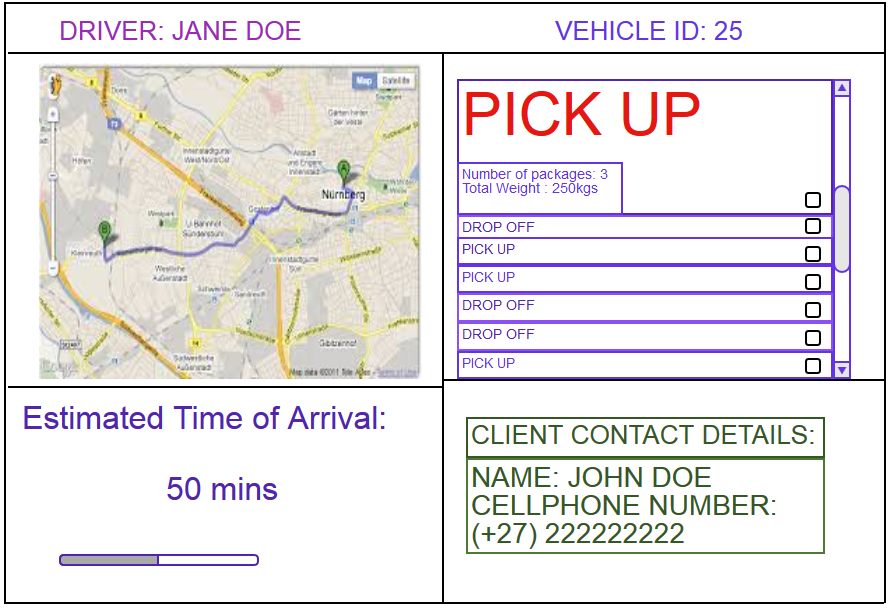
\includegraphics[width=5in]{pictures/driver.png}
\caption{The driver interface}
\label{Driver}
\end{figure}

\subsubsection{The dispatcher view}
The following figure shows you the dispatcher view before the dispatcher runs the algorithm to assign packages to drivers and routes.
\begin{figure}[h!]
\centering
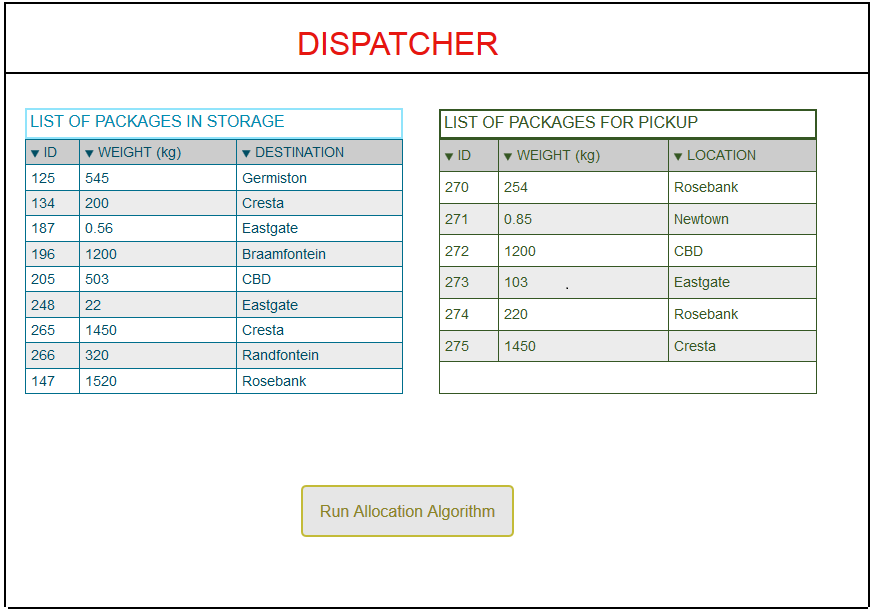
\includegraphics[width=3.5in]{pictures/dispatcherBefore.png}
\caption{The dispatcher interface before running the allocation algorithm}
\label{DispatcherBefore}
\end{figure}

The following figure shows you the dispatcher view after the dispatcher runs the algorithm to assign packages to drivers and routes.
\begin{figure}[h!]
\centering
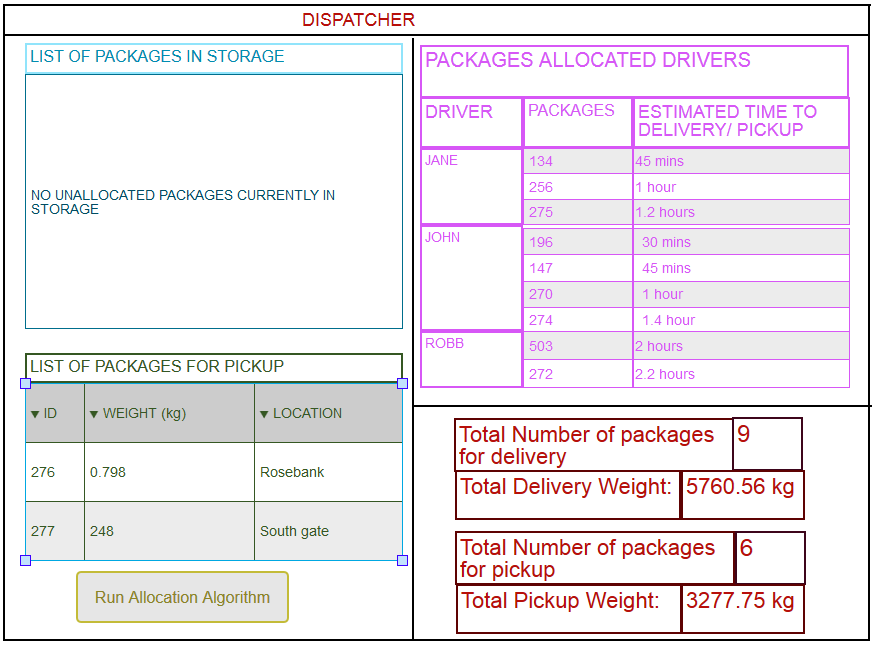
\includegraphics[width=3.5in]{pictures/dispatcher.png}
\caption{The dispatcher interface}
\label{Dispatcher}
\end{figure}


\subsubsection{The receiver view before user submits}
In order for the receiver to track the progress of their package they have to enter the package notification sent to them via email notification. Figure \ref{ReceiverBefore} shows the page where the user enters their package id.
\begin{figure}[h!]
\centering
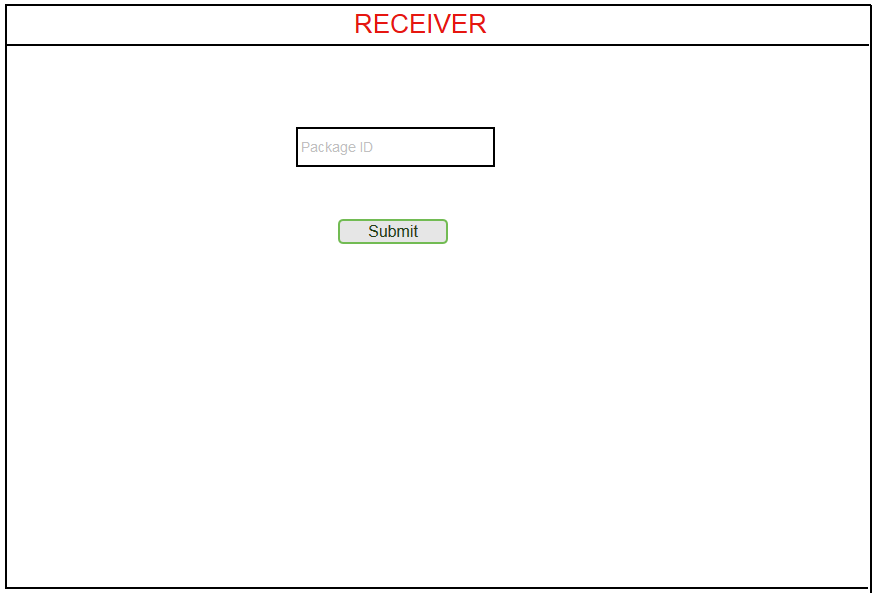
\includegraphics[width=3.5in]{pictures/receiverBefore.png}
\caption{The receiver interface}
\label{ReceiverBefore}
\end{figure}

\subsubsection{The receiver view after the user submits}
Figure \ref{ReceiverAfter} shows the interface the receiver sees after they have entered their package details. This view shows the package details and estimated time of delivery.
\begin{figure}[h!]
\centering
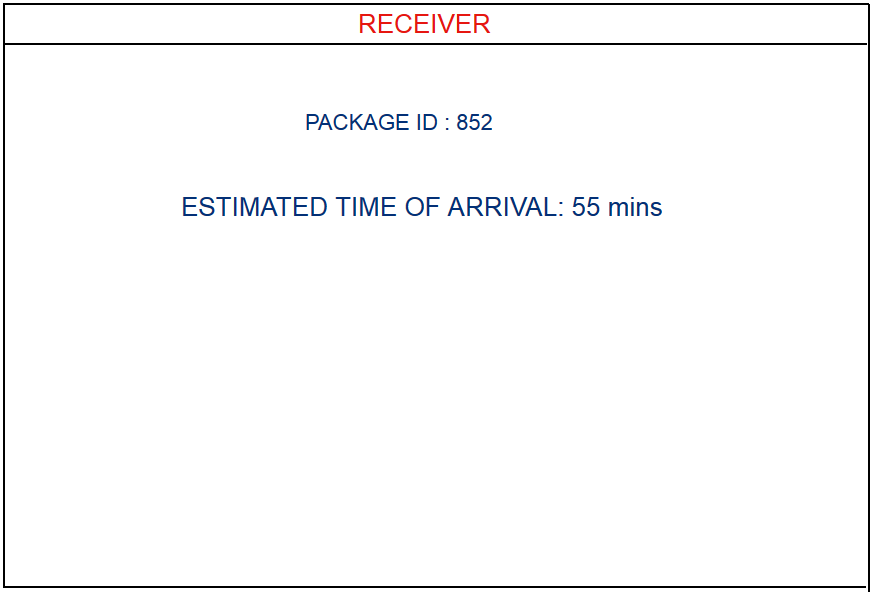
\includegraphics[width=3.5in]{pictures/receiverAfter.png}
\caption{The receiver interface after the user submits query} 
\label{ReceiverAfter}
\end{figure}

\subsubsection{The sender view}
Figure \ref{Sender} shows the sender view.
\begin{figure}[h!]
\centering
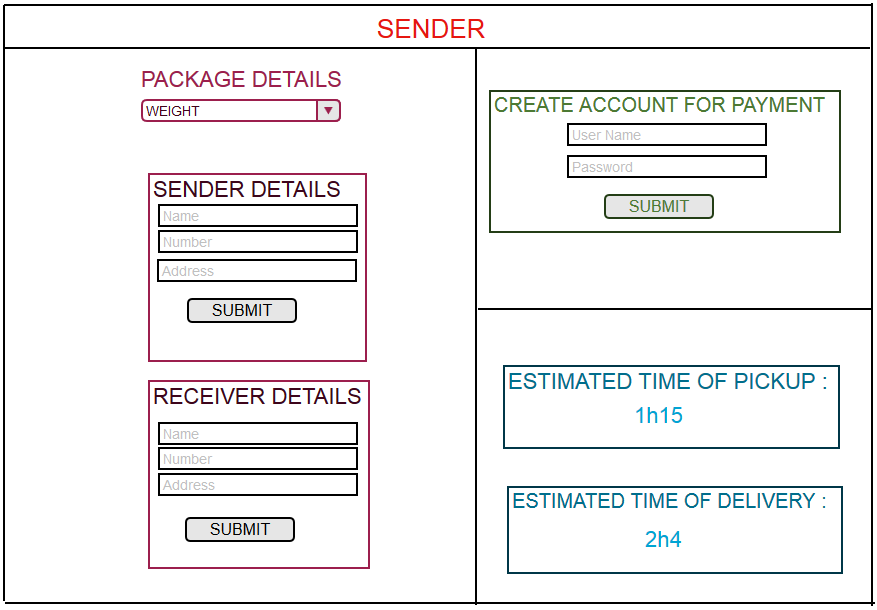
\includegraphics[width=3.5in]{pictures/sender.png}
\caption{The sender interface}
\label{Sender}
\end{figure}

\subsubsection{The Accounts officer view}
Figure \ref{Sender} shows the Accounts officer view.
\begin{figure}[h!]
\centering
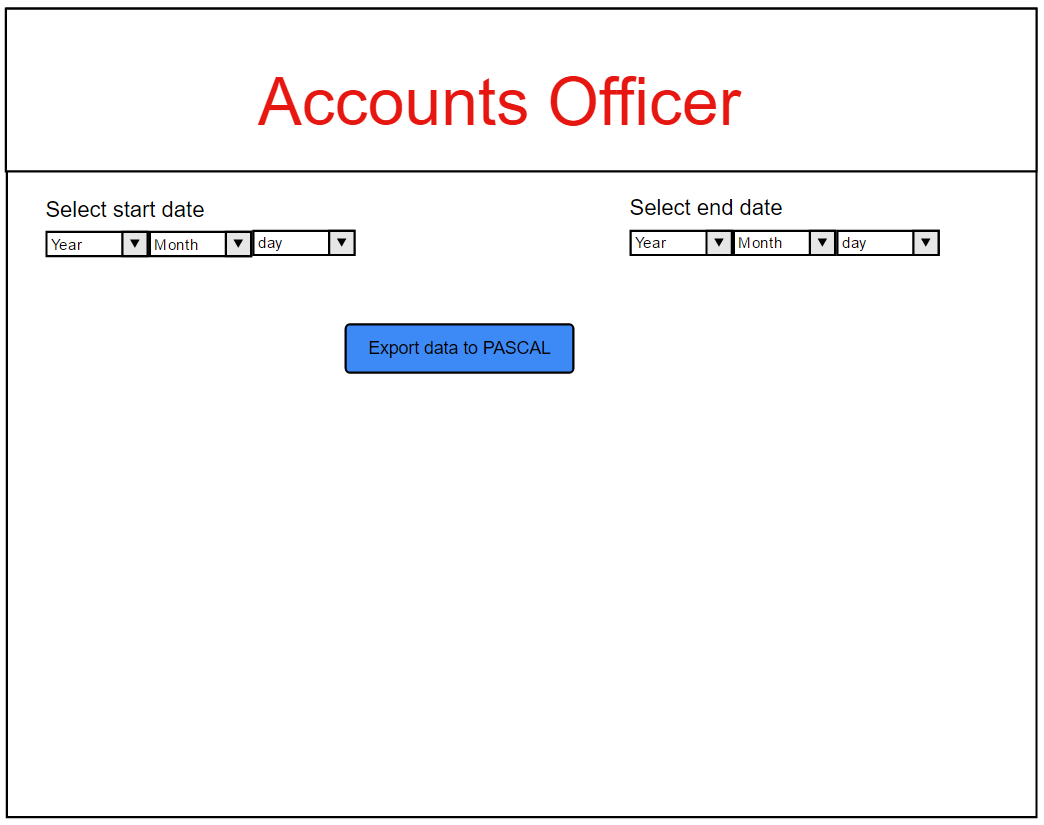
\includegraphics[width=3.5in]{pictures/accounts.png}
\caption{The accounts officer interface}
\label{Sender}
\end{figure}

\subsubsection{The CEO view}
Figure \ref{Sender} shows the CEO view.
\begin{figure}[h!]
\centering
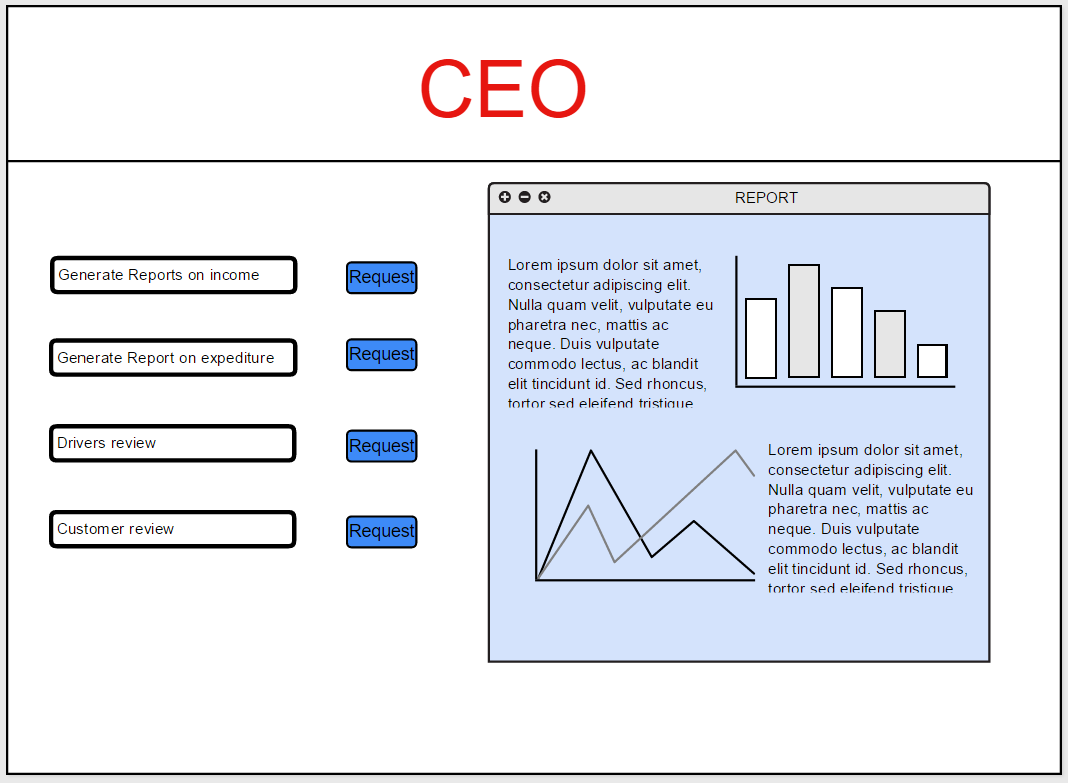
\includegraphics[width=3.5in]{pictures/CEO.png}
\caption{The CEO view}
\label{Sender}
\end{figure}

\subsubsection{The Operational officer view}
Figure \ref{Sender} shows the Operational officer view.
\begin{figure}[h!]
\centering
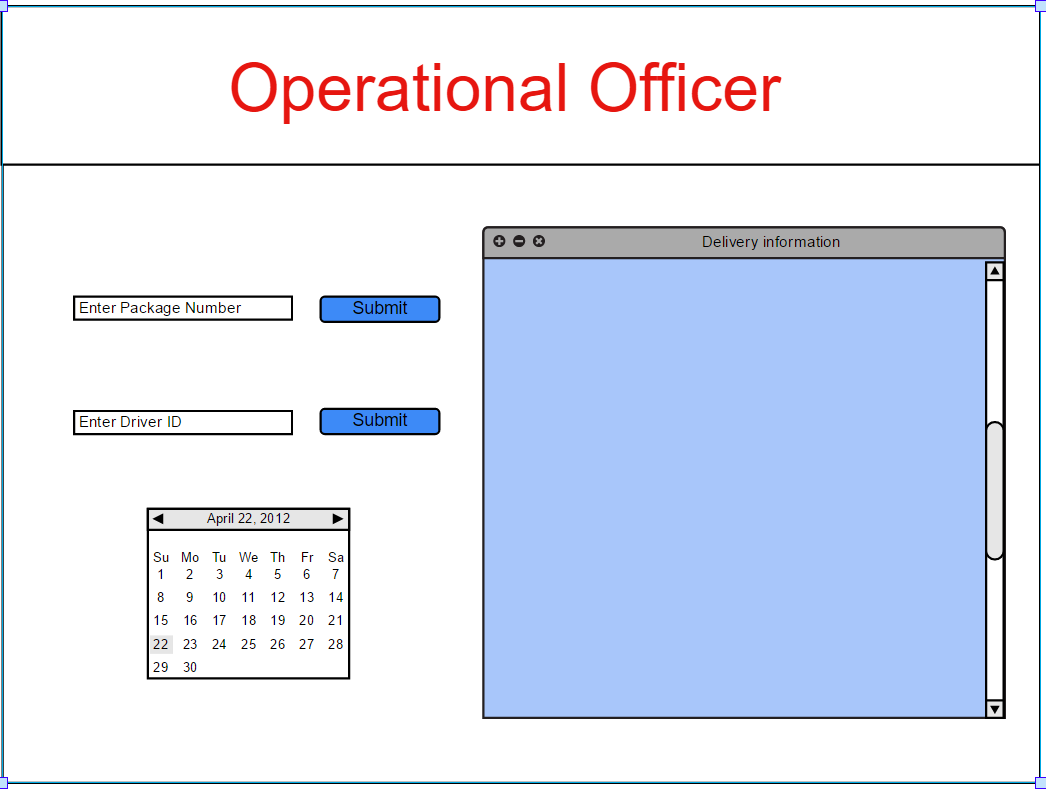
\includegraphics[width=3.5in]{pictures/operational.png}
\caption{The operational officer interface}
\label{Sender}
\end{figure}

\subsubsection{The system administrator view}
Figure \ref{Sender} shows the system administrator view.
\begin{figure}[h!]
\centering
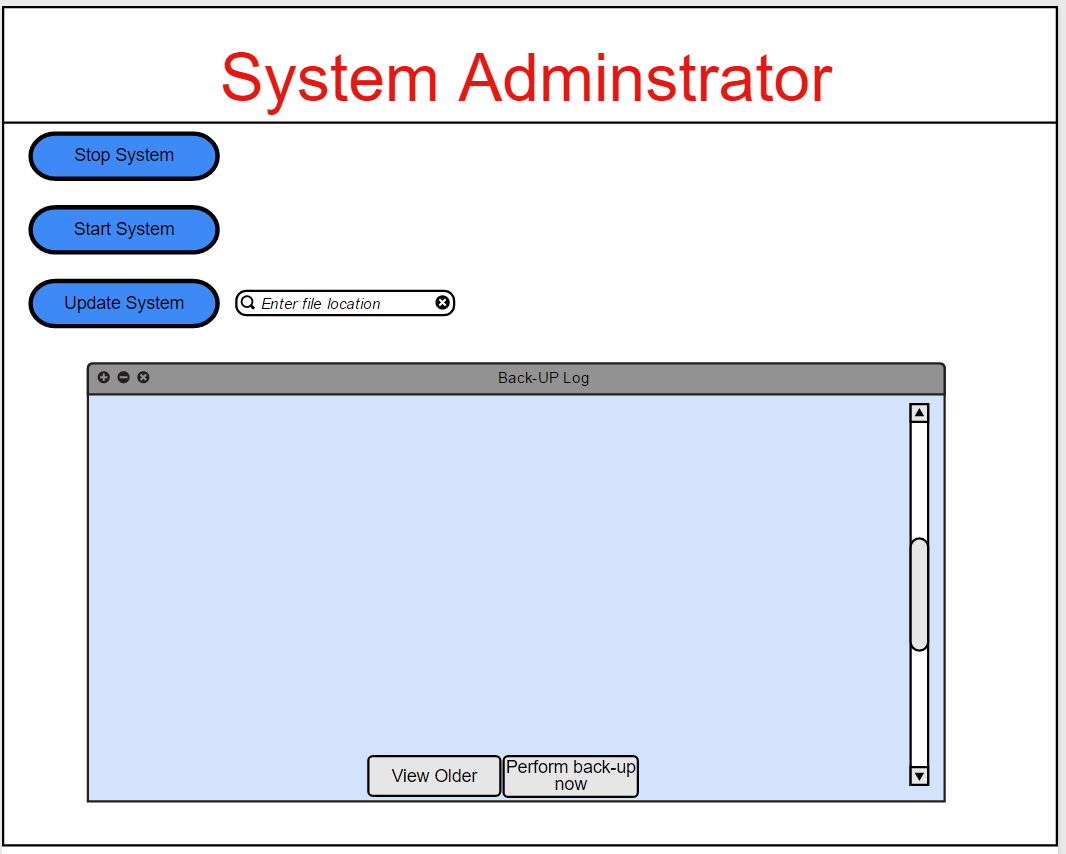
\includegraphics[width=3.5in]{pictures/admin.png}
\caption{The system administrator interface}
\label{Sender}
\end{figure}

\subsubsection{The Vehicle maintenance view}
Figure \ref{Sender} shows the vehicle maintenance view.
\begin{figure}[h!]
\centering
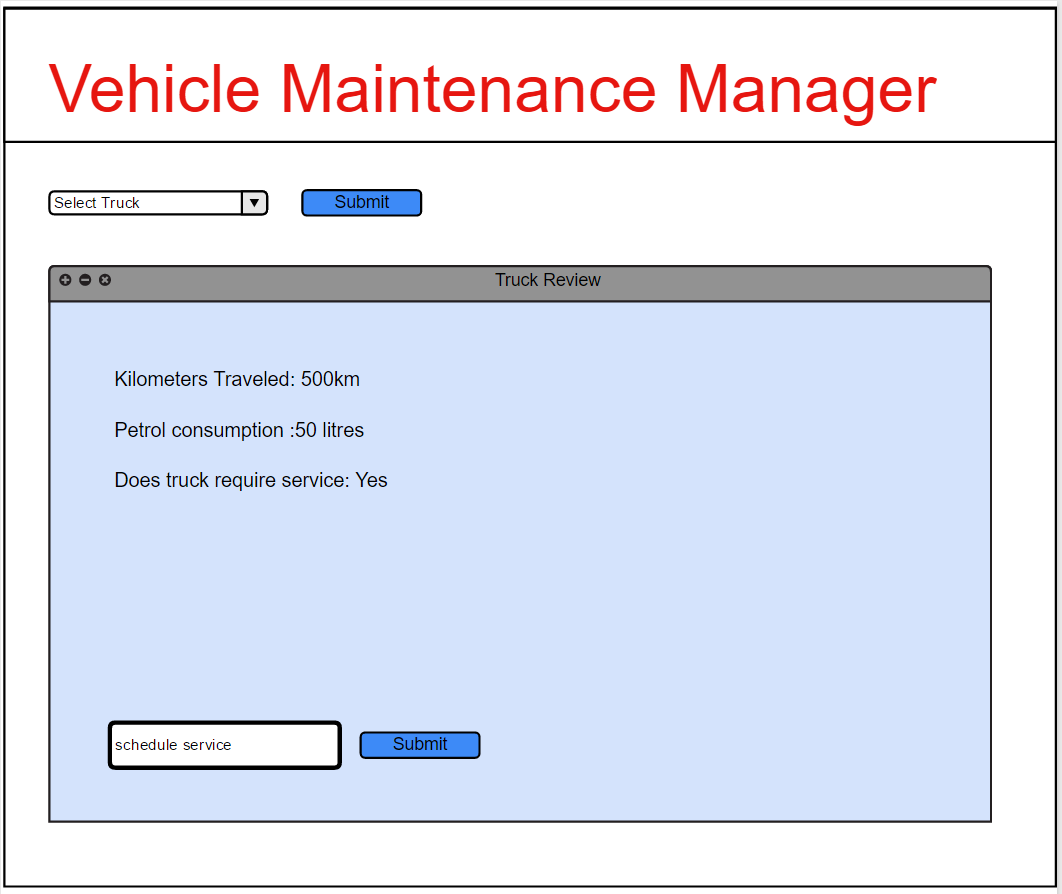
\includegraphics[width=3.5in]{pictures/vehicle.png}
\caption{The vehicle maintenance manager interface}
\label{Sender}
\end{figure}

\subsection{Hardware interfaces}
\begin{itemize}
			\item Mobile phone/ desktop/tablet
\end{itemize}

\subsection{Software interfaces}
	\begin{itemize}
		\item Latest version of preferred web browser, preferably Chrome.
	\end{itemize}
\subsection{Communication interfaces}
	\begin{itemize}
		\item Internet connection
		\item Email notifications
		\item Telephone calls
		\item SMS notification
	\end{itemize}

\section{System Features}


\subsection{Tracking of parcels}
\subsubsection{Introduction/Purpose of feature}

Parcel tracking enables the manager of the depot to see the status and locations of all parcels to be collected or delivered. This can be useful for when parcels go missing and they need to be found as the parcel would have been lost after its last known location. Parcel tracking also helps the dispatchers ensure that the correct parcels are in the correct vehicles so that deliveries can be made in the shortest possible time. The customers also benefit from this feature as they may track the parcel from its tracking number.
\subsubsection{Stimulus/Response Sequence}
The parcel is given its location  from its point of origin, this is the pick up point that is logged when a driver firsts collects the parcel. The second location of all parcels will be the dispatch warehouse where parcels are stored and sorted. The parcel will then be sent to a delivery vehicle. As the delivery vehicle makes collections/deliveries, the parcels location will be updated. 
\subsubsection{Associated Functional requirements}
This feature requires an internet enable device for both the driver to relay the parcels position and the user to locate where the parcel is. These devices will then need to connect to a centralised server which is responsible for processing and storing all data requests. 
\subsection{Tracking of vehicles}
\subsubsection{Introduction/Purpose of feature}
This feature allows the manager to have full access to the location of all vehicles in order to determine whether the drivers are following the right paths, no unnecessary stops are made and that all delays are accounted for. This can help the manager pick up any faults in the user algorithm and make the necessary changes. This is also useful for determining the location of parcels as they can take their location data from the location of the vehicle in which they are contained.
\subsubsection{Stimulus/Response Sequence}
When the driver logs on to the system, the location of the driver is continuously fed through the internet to the companies servers. This is an automatic process that happens in the background when a driver is logged in. 
\subsubsection{Associated Functional requirements}
This feature requires an internet enabled device that also has a GPS system to calculate its position, network triangulation can also be used but this should be avoided. The device would then connect to a server via the internet which is responsible for processing and storing all data requests.
\subsection{Determine shortest distance route}
\subsubsection{Introduction/Purpose of feature}
The shortest distance route is used when a list of deliveries and pick up are acquired for  an individual vehicle. A shortest distance algorithm which is based on Dijkstra's algorithm will be used. This algorithm will calculate the shortest distance between the first stop, the last stop and all the points in between. This will determine the path for the driver to take when making both pick ups and deliveries.
\subsubsection{Stimulus/Response Sequence}
The list of destinations are determined at the start of the day when the dispatcher runs the allocation algorithm. The system will then divide the locations into zones depending on the delivery vehicles available, i.e. each vehicle is responsible for its own zone. The system will then use the shortest distance algorithm to calculate the shortest distance for the driver between all points. This will be pushed to the driver's profile which is then accessible from an internet connected device.
\subsubsection{Associated Functional requirements}
This requires processing power from a server to calculate all possible driving routes and determine the shortest route. The more efficient algorithm will lessen the load on servers. The driver will then have access to the information on the server through an internet connected device.
\subsection{Determine the vehicle certain packages go into}
\subsubsection{Introduction/Purpose of feature}
To optimise efficiency and be cost effective the system should be able to ensure that packages that are to be delivered or collected from the same area are in the same truck without exceeding the maximum weight limits placed on a truck. 
\subsubsection{Stimulus/Response Sequence}
\begin{itemize}
			\item The dispatcher has to press the Run Allocation Algorithm button. This results in the algorithms which determine which truck the package has to be placed in being run in the background. The inputs to the algorithms include destination/location of package, weight of package and truck specifications such as maximum weight allowed.
			\item When a user enters a package into the system for pick up the allocation algorithms will be run to determine which truck will pick up the package.
\end{itemize}
	 
\subsubsection{Associated Functional requirements}
\begin{itemize}
			\item The packages that will be allocated vehicles are both packages that are already at the storage house and packages that users have entered into the system for pick up.
			\item When a driver receives a route at the beginning of their shift they will not be allocated extra packages even if the package to be collected is in the vicinity of the driver's route. All routes and time tables are determined when drivers are allocated trucks at the start of their shift.
\end{itemize}
	
\subsection{Allocate a driver to a vehicle}
\subsubsection{Introduction/Purpose of feature}
When a vehicle has been allocated packages and the allocation is deemed complete; a driver will then be allocated to drive the vehicle.  All drivers working on that day should be allocated at least 3 hours worth of driving work in a day. Drivers and vehicles are allocated according to availability. No driver has a specific vehicle allocated to them permanently.
\subsubsection{Stimulus/Response Sequence}
The dispatcher has to press the Run Allocation Algorithm button. After all the packages have been assigned trucks; the allocate drivers to trucks algorithm will be run. The inputs to this algorithm include the status of truck allocation and the available drivers list. 
\subsubsection{Associated Functional requirements}
\begin{itemize}
			\item This is only run when the algorithm for allocating truck has been run.
			\item Drivers are allocated depending on availability not how often they drive a certain vehicle.
\end{itemize}
	

\subsection{Determine date and time of package pickup}
\subsubsection{Introduction/Purpose of feature}
Depending on the route a package has been allocated to, it will be assigned a date and time of pickup. The further down a route a package is located the longer it will take for it to be delivered or collected.  
\subsubsection{Stimulus/Response Sequence}
\begin{itemize}
			\item The dispatcher has to press the Run Allocation Algorithm button. After all the packages have been assigned trucks depending on the location of the package, that is, how far down the route it is, a time will be allocated to it. 
			\item When a user enters a package into the system for pick up the date and time algorithm will be run just after the vehicle allocation algorithm is complete.
\end{itemize}

 
\subsubsection{Associated Functional requirements}
\begin{itemize}
\item This allocation has to be done just after the packages have been allocated trucks.
\end{itemize}
			

\subsection{Determine date and time of delivery}
\subsubsection{Introduction/Purpose of feature}
Depending on the route a package has been allocated to it will be assigned a date and time of delivery. The further down a route a package is located the longer it will take for it to be delivered or collected.  
\subsubsection{Stimulus/Response Sequence}
\begin{itemize}
			\item The dispatcher has to press the Run Allocation Algorithm button. After all the packages have been assigned trucks depending on the location of the package, that is, how far down the route it is, a time will be allocated to it.  
			\item When a user enters a package into the system for pick up the date and time algorithm will be run just after the vehicle allocation algorithm is complete.
\end{itemize}
	 

\subsubsection{Associated Functional requirements}

\begin{itemize}
			\item This allocation has to be done just after the packages have been allocated trucks. 
\end{itemize}

	

\subsection{Store payment information}
\subsubsection{Introduction/Purpose of feature}
In order for a user to complete the process of being able to send a parcel they will first have to create an account. When an account is created, the user has to store their payment details.
\subsubsection{Stimulus/Response Sequence}
\begin{itemize}
			\item The sender presses on the button create an account 
			\item The sender then enters all their information 
			\item The sender then presses the button submit which creates an account 
\end{itemize}
	
\subsubsection{Associated Functional requirements}
This has to be done before a sender can send anything. A database has to be created which can store all the information

\subsection{Store client details}
\subsubsection{Introduction/Purpose of feature}
In order for a user to complete the process of being able to send a parcel they will first have to create an account. When an account is created, the user has to store their personal details.
\subsubsection{Stimulus/Response Sequence}
\begin{itemize}
			\item The sender presses on the button create an account
			\item The sender then enters all their information 
			\item The sender then presses the submit button which creates an account 
\end{itemize}
	

\subsubsection{Associated Functional requirements}
This has to be done before a sender can actually send anything. A database has to be created which can store all the information

\subsection{Package Storage and Package Identification}
\subsubsection{Introduction/Purpose of feature}

Each package is given a unique tracking ID when the sender requests a pick up. This tracking ID is used to identify the package through its various stages i.e. storage or delivery.


\subsubsection{Stimulus/Response Sequence}
\begin{itemize}
\item The sender enters and submits the package details.
\item The sender enters and submits the receiver's address.
\item The sender is charged on submission.
\end{itemize}
\subsubsection{Associated Functional requirements}
\begin{itemize}
\item A database to store the package details.
\item A database to store addresses.
\item A server that will take care of the payments
\end{itemize}


\subsection{Send automated email notifications to clients}
\subsubsection{Introduction/Purpose of feature}

A tracking ID is sent to the receiver via email. The tracking number can be used to view information on location and status of the package.

\subsubsection{Stimulus/Response Sequence}
\begin{itemize}
\item The client needs to click on the web link sent to them via email to access the receiver dashboard.
\item Enter their tracking ID and submit.
\end{itemize}
\subsubsection{Associated Functional requirements}
\begin{itemize}
\item Package storage and identification.
All sender functionality must work before the receiver functionality can be implemented.
\end{itemize}

\subsection{Inventory management}
\subsubsection{Introduction/Purpose of feature}
To make sure that there is enough storage space in the store room for the packages to be stored. This will determine the estimated time of pickup and delivery due to the backlog in the storehouse.
\subsubsection{Stimulus/Response Sequence}
\begin{itemize}
\item The sender should press submit after creating the payment account.
\end{itemize}
\subsubsection{Associated Functional requirements}
\begin{itemize}
\item Package storage and identifier.
\item A database to store the package details.
\item A server that will take care of the payments.
\end{itemize}


\section{Performance Requirements}
\begin{itemize}
			\item Loading times
			\item Algorithm run times 
			\item The number of users at the same time 
\end{itemize}
	
\section{Design Constraints}
\begin{itemize}
			\item Time
			\item Resources (using only open source software) 
			\item Data Acquisition
			\item Domain expert knowledge missing  
\end{itemize}
	
\section{Software system attributes}
\subsection{Reliability}
In order to establish the reliability of the software at a time of delivery, the following factors are required:
\begin{itemize}
			\item Testing should be carried out concurrently with the writing of the code
			\item The client should be part of the design and testing processes
			  
\end{itemize}
	

\subsection{Availability}
This will not be defined for this project.
\subsection{Security}
 A main feature of the website is that depending on the person who is using it (sender ,dispatcher ,driver), they should only be able to access their relevant part. Therefore code that restricts communications between these different sections needs to be implemented.
Cryptographic techniques should be used to protect the data. However this is beyond the scope of this project.
\subsection{Maintainability}

The functionality should be separated into different classes according to it's role.The code will be extensively commented and documented using Doxygen.

\subsection{Portability}
The system is meant to have one centralised server which handles all user requests. The system can be accessed by any internet enabled device as they only access a webpage.


%\begin{align} 
%\begin{split}
%(x+y)^3 	&= (x+y)^2(x+y)\\
%&=(x^2+2xy+y^2)(x+y)\\
%&=(x^3+2x^2y+xy^2) + (x^2y+2xy^2+y^3)\\
%&=x^3+3x^2y+3xy^2+y^3
%\end{split}					
%\end{align}



%------------------------------------------------





%\paragraph{Heading on level 4 (paragraph)}
%
%\lipsum[6] % Dummy text
%
%%----------------------------------------------------------------------------------------
%%	PROBLEM 2
%%----------------------------------------------------------------------------------------
%
%\section{Lists}
%
%%------------------------------------------------
%
%\subsection{Example of list (3*itemize)}
%\begin{itemize}
%	\item First item in a list 
%		\begin{itemize}
%		\item First item in a list 
%			\begin{itemize}
%			\item First item in a list 
%			\item Second item in a list 
%			\end{itemize}
%		\item Second item in a list 
%		\end{itemize}
%	\item Second item in a list 
%\end{itemize}
%
%%------------------------------------------------
%
%\subsection{Example of list (enumerate)}
%\begin{enumerate}
%\item First item in a list 
%\item Second item in a list 
%\item Third item in a list
%\end{enumerate}
%
%%----------------------------------------------------------------------------------------

\end{document}